\section{Padrão arquitetural Model-View-Controller(MVC)}

    \par Esta seção tem como objetivo, explorar o MVC desde o seu surgimento na Xerox PARC até as versões mais modernas utilizadas do desenvolvimento web. Essa abordagem ajudará a entender por que mesmo depois de quatro décadas o MVC ainda vem sendo relevante para o desenvolvimento de software, o que corrobora para entender-se como implementar os princípios da arquitetura limpa em seu contexto.
    
    \subsection{Contexto histórico}
    
        \par O padrão arquitetural Model-View-Controller (MVC) foi desenvolvido em 1978 por Trygve Reenskaug enquanto o mesmo trabalhava na Xerox PARC, com o objetivo de criar sistemas de informação que refletissem os modelos mentais dos usuários, promovendo uma interação intuitiva por meio de inspeção e edição de dados \cite[p.~1]{artigo:reenskaug:2003}. 
        
        \par Ainda nesse contexto, a sua implementação foi realizada inicialmente no ambiente Smalltalk, e foi formalizada como um padrão por Reenskaug em notas técnicas publicadas em maio e dezembro de 1979, essa notas estabeleceram as bases do padrão \cite{artigo:reenskaug:1979}.
        
        \par Quanto a validação e a demonstração de eficacia do padrão MVC, as mesmas vieram de um experimento no Xerox PARC, envolvendo um sistema de planejamento para uma fábrica de semicondutores, dessa forma mostrando a sua aplicabilidade prática \cite{artigo:reenskaug:2003}.
        
        \par Com a evolução tecnológica, o MVC foi adaptado para interfaces mais complexas e posteriormente inspirou frameworks modernos, como o ASP.NET MVC, que foi lançado no ano de 2009 \cite{artigo:deacon:2009}. Nesse sentido é notável  que o Smalltalk foi o responsável pela criação do padrão MVC, que posteriormente se tornou amplamente adotado em sistemas orientados a objetos \cite{artigo:deacon:2009}.
        
    \subsection{Definição}
        \par O MVC é um padrão arquitetural que separa o software em três camadas, a camada que contem lógica do domínio da aplicação chamada Model, a camada que é responsável pela apresentação dos dados chamada View e a camada responsável por controlar as interações do usuário com a aplicação chamada Controller, assim promovendo modularidade, reutilização e manutenção do sistema\cite{artigo:reenskaug:2003}.

        \par Nesse contexto de definição de conceitos, nota-se que o coração do padrão MVC não é a separação técnica entre Model, View e Controller, mas a garantia de que o Model espelhe o modelo mental do usuário \cite{artigo:reenskaug:2003}. 
        
        \par Isso significa que, ao interagir com o sistema, o usuário não está lidando com tabelas de banco de dados ou JSON, mas com representações digitais de conceitos que já fazem parte do seu entendimento (ex.: 'projetos', 'tarefas', 'prazos'). Essa abordagem, inspirada em psicologia cognitiva e em linguagens de modelagem como UML, foi o que diferenciou o MVC de padrões anteriores \cite{artigo:reenskaug:2003}.

        \begin{figure}[H] % O [H] exige o uso do pacote float (veja abaixo)
            \centering
            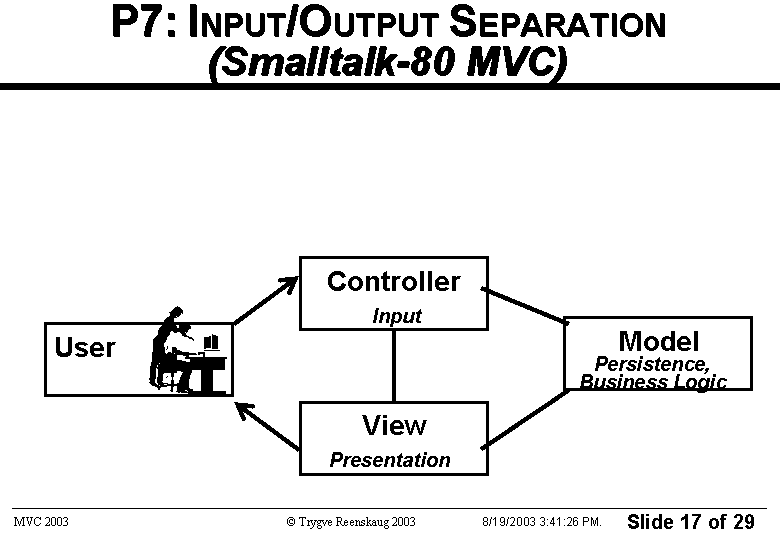
\includegraphics[width=0.8\textwidth]{figuras/figura_mvc_1.png}
            \caption{Modelo de colaboração UML da solução Smalltalk-80.}
            \label{fig:figura_mvc_1}
            \newcommand{\source}{Fonte: \cite{artigo:reenskaug:2003}}
        \end{figure}

        \subsubsection{Model}
            \par A camada Model representa o núcleo do domínio da aplicação, encapsulando tanto os dados quanto as regras de negócio que comandam o comportamento do sistema. Ela deve manter-se completamente independente das questões relacionadas à interface do usuário, não contendo qualquer referência direta ou conhecimento sobre como os dados são apresentados ou manipulados externamente \cite{artigo:deacon:2009}
            
            \par Esta camada é composta por entidades que modelam o problema em questão, como classes representando clientes, transações financeiras ou reservas, permanecendo estável mesmo quando as interfaces de usuário sofrem modificações significativas \cite{artigo:deacon:2009}. 
            
            \par A literatura ainda explica uma distinção importante entre o Modelo de Domínio (Md), que contém a lógica essencial do negócio, e o Modelo de Aplicação (Ma), que atua como mediador entre o núcleo do sistema e as camadas de apresentação \cite{artigo:deacon:2009}.
            
        \subsubsection{View}
            \par A camada View é responsável pela apresentação dos dados ao usuário final, assumindo o papel de interface através da qual a interação com o sistema ocorre. Uma mesma aplicação pode possuir múltiplas Views para um único Model, permitindo diferentes formas de visualização e interação com os mesmos dados subjacentes. Estas podem variar desde interfaces gráficas sofisticadas (GUIs) até linhas de comando textuais (CLIs) ou mesmo APIs para integração com outros sistemas \cite{artigo:deacon:2009}.
            
            \par A View possui conhecimento sobre a existência e estrutura do Model, acessando seus dados para exibição, mas o inverso não é verdadeiro - o Model permanece completamente alheio às suas Views. Esta relação unidirecional é fundamental para manter o baixo acoplamento do sistema, permitindo que as Views sejam modificadas ou expandidas sem impactar a camada de domínio da aplicação \cite{artigo:deacon:2009}.

        \subsubsection{Controller}
            \par O Controller atua como o componente responsável por processar as entradas do usuário, traduzindo ações físicas (como cliques de mouse ou pressionamentos de tecla) em comandos significativos para o sistema. Em muitas implementações modernas, observa-se uma tendência de fusão entre View e Controller, resultando em um componente único frequentemente denominado Delegate \cite{artigo:deacon:2009}.
            
            \par Ele ainda mantém suas características específicas vistas no modelo tradicional, incluindo sua natureza dependente de plataforma, pois deve lidar com as particularidades do sistema operacional subjacente, e seu caráter essencialmente processual, focando na interpretação de eventos sem armazenar estado permanente \cite{artigo:deacon:2009}.
            
        \subsubsection{A comunicação entre os componentes}
        
            \par A comunicação entre estes componentes segue padrões bem definidos que preservam a separação de conceitos. As Views se comunicam com o Model através de mensagens, geralmente mediadas pelo Modelo de Aplicação quando este está presente, para solicitar atualizações ou acesso a dados \cite{artigo:deacon:2009}.
            
            \par O fluxo inverso, onde mudanças no Model precisam ser refletidas nas Views, ocorre através de mecanismos de notificação por eventos, garantindo que o Model permaneça independente de suas Views \cite{artigo:deacon:2009}.
            
            \par Já os Controllers, por sua vez, interceptam as interações do usuário com a aplicação, decidindo quais ações vão ser disparadas na View ou no Model, sem no entanto assumir responsabilidades que pertençam a estes componentes, mantendo assim sua responsabilidade bem definida \cite{artigo:deacon:2009}.
            
        \subsubsection{Diferenciais}
            \par A arquitetura MVC oferece diferencias significativos para o desenvolvimento e manutenção de sistemas de software complexos. Ao isolar a lógica de negócio das preocupações com interface do usuário, torna-se possível modificar ou expandir as camadas de apresentação sem afetar o núcleo do sistema, assim como reutilizar o mesmo Model em diferentes contextos e plataformas \cite{artigo:deacon:2009}.
            
            \par A comunicação baseada em eventos e o princípio de dependência unidirecional entre os componentes contribuem para a criação de sistemas mais flexíveis, coesos e fáceis de manter, características essenciais em ambientes onde os requisitos estão sujeitos a mudanças frequentes \cite{artigo:deacon:2009}.

    \subsection{Padrão MVC no Smalltalk-80}

        \par Conforme já mostrado no presente trabalho o MVC tem sua origem no Smalltalk-80, tendo isso em vista podemos detalhar como funcionava a implementação inicial desse padrão trazendo bons pararelos para as implementações mais modernas desse padrão.
    
        \par O padrão MVC estabeleceu uma arquitetura inovadora para sistemas interativos \cite{artigo:reenskaug:2003}. No Smalltalk-80, o Model representava a base do sistema, encapsulando os dados e o comportamento essencial do domínio da aplicação \cite{artigo:reenskaug:2003}. A View assumia a responsabilidade pela apresentação visual dos dados contidos no Model, podendo existir múltiplas Views para um mesmo Model, como já mencionado anteriormente \cite{artigo:reenskaug:2003}.
        
        \par O Controller funcionava como mediador entre as ações do usuário e o sistema, interpretando eventos de entrada e traduzindo-os em operações específicas \cite{artigo:reenskaug:2003}. Em componentes mais simples, como as barras de rolagem, os papéis de View e Controller frequentemente se fundiam em um único objeto \cite{artigo:reenskaug:2003}.

        \par Nesse mesmo contexto, o mecanismo de sincronização entre Model e View operava através do padrão Observer, onde modificações no Model automaticamente notificavam todas as Views registradas para o mesmo \cite{artigo:reenskaug:2003}. Com o objetivo de otimizar o desempenho da aplicação, implementavam-se técnicas como transações que agrupavam múltiplas alterações antes de propagá-las às Views \cite{artigo:reenskaug:2003}.
        
        \par Além disso, a arquitetura ainda previa o conceito de Tools, que coordenavam conjuntos de Editores (Views) para tarefas complexas, garantindo consistência na interface \cite{artigo:reenskaug:2003}. 
        
        \par Esta implementação do MVC no Smalltalk-80 serviu como base, definindo os princípios fundamentais de separação de preocupações que influenciaram profundamente o desenvolvimento de interfaces gráficas no futuro \cite{artigo:reenskaug:2003}
            
    \subsection{Padrão MVC-WEB}
    
        \par O padrão MVC-Web surge como uma adaptação do tradicional Model-View-Controller (MVC) para o contexto de aplicações web, onde a arquitetura cliente-servidor e o protocolo HTTP introduzem desafios distintos em relação aos sistemas desktop originais \cite{inproceedings:grove:2011}.
        
        \par Enquanto o MVC clássico foi concebido para ambientes interativos como o Smalltalk-80, o MVC-Web reflete as mudanças necessárias para lidar com a natureza stateless da web, a separação física entre cliente e servidor e a necessidade de gerenciamento explícito do fluxo de navegação \cite{inproceedings:grove:2011}.

        \subsubsection{Model}
        
            \par No MVC-Web, o Model mantém sua função central de gerenciar o estado da aplicação e suas regras de negócio mas com adaptações significativas:

            \begin{itemize}
                \item Persistência de Dados: Diferentemente do Smalltalk, onde o modelo era persistente na memória, em frameworks web como Rails ou ASP.NET, o modelo frequentemente interage com bancos de dados, usando padrões como Active Record ou ORM (Mapeamento Objeto-Relacional) \cite{inproceedings:grove:2011}.
                
                \item Transações e Lógica de Negócio: O modelo continua responsável por executar operações críticas, mas sua comunicação com as views não ocorre mais via Observer (como no padrão original). Em vez disso, o controller atua como intermediário \cite{inproceedings:grove:2011}.
                
                \item Interfaces Externas: Em aplicações modernas, o modelo também pode integrar APIs externas ou serviços web, expandindo sua função além do armazenamento local \cite{inproceedings:grove:2011}.
            \end{itemize}


        \subsubsection{View}
    
            \par A View no MVC-Web assume um papel híbrido, combinando renderização server-side com interatividade client-side:

            \begin{itemize}
                \item Templates Dinâmicos: Frameworks como Rails e ASP.NET usam templates HTML com código embutido para gerar páginas dinamicamente \cite{inproceedings:grove:2011}.

                \item Interações no lado do cliente: Com tecnologias como JavaScript e Ajax, a view pode realizar validações, atualizações parciais e outras operações sem recarregar a página, assumindo funções que, no MVC original, eram do modelo ou controller \cite{inproceedings:grove:2011}.

                \item Separação Menos Rígida: Enquanto no Smalltalk a view era passiva (só exibia dados), no MVC-Web ela pode conter lógica de apresentação e até mesmo regras de negócio simples (como validação de formulários), o que desafia a pureza do padrão \cite{inproceedings:grove:2011}.
            \end{itemize}
        
       
        \subsubsection{Controller}
        
        \par O Controller no MVC-Web sofre as mudanças mais radicais, principalmente devido ao Front Controller, um padrão arquitetônico que centraliza o tratamento de requisições HTTP:

        \begin{itemize}
            \item Front Controller: Frameworks como (ASP.NET MVC, Rails, Struts) implementam esse padrão, onde um único componente (como o Router no Rails) centraliza o roteamento de requisições HTTP para controllers específicos \cite{inproceedings:grove:2011}.

            \item Ações e Fluxo de Navegação: Cada método de um controller (ex: UsersController@create) corresponde a uma ação (como criar um usuário). O controller decide qual view exibir com base no resultado (ex: redirecionar após um sucesso ou mostrar um erro) \cite{inproceedings:grove:2011}.

            \item Validação e Preparação de Dados: O controller filtra e valida parâmetros da requisição (como dados de formulários), delegando apenas a lógica de negócio ao modelo \cite{inproceedings:grove:2011}.            
        \end{itemize}